%% Artikelvorlage unter Verwendung der Artikelklasse des KOMA-Script %%
%% Basierend auf einer TeXNicCenter-Vorlage von Mark M�ller          %%
%%%%%%%%%%%%%%%%%%%%%%%%%%%%%%%%%%%%%%%%%%%%%%%%%%%%%%%%%%%%%%%%%%%%%%%

% W�hlen Sie die Optionen aus, indem Sie % vor der Option entfernen  
% Dokumentation des KOMA-Script-Packets: scrguide

%%%%%%%%%%%%%%%%%%%%%%%%%%%%%%%%%%%%%%%%%%%%%%%%%%%%%%%%%%%%%%%%%%%%%%%
%% Optionen zum Layout des Artikels                                  %%
%%%%%%%%%%%%%%%%%%%%%%%%%%%%%%%%%%%%%%%%%%%%%%%%%%%%%%%%%%%%%%%%%%%%%%%
\documentclass[%
%a5paper,							% alle weiteren Papierformat einstellbar
%landscape,						% Querformat
10pt,								% Schriftgr��e (12pt, 11pt (Standard))
%BCOR1cm,							% Bindekorrektur, bspw. 1 cm
%DIVcalc,							% f�hrt die Satzspiegelberechnung neu aus
%											  s. scrguide 2.4
%twoside,							% Doppelseiten
%twocolumn,						% zweispaltiger Satz
%halfparskip*,				% Absatzformatierung s. scrguide 3.1
%headsepline,					% Trennline zum Seitenkopf	
%footsepline,					% Trennline zum Seitenfu�
%titlepage,						% Titelei auf eigener Seite
%normalheadings,			% �berschriften etwas kleiner (smallheadings)
%idxtotoc,						% Index im Inhaltsverzeichnis
%liststotoc,					% Abb.- und Tab.verzeichnis im Inhalt
%bibtotoc,						% Literaturverzeichnis im Inhalt
%abstracton,					% �berschrift �ber der Zusammenfassung an	
%leqno,   						% Nummerierung von Gleichungen links
%fleqn,								% Ausgabe von Gleichungen linksb�ndig
%draft								% �berlangen Zeilen in Ausgabe gekennzeichnet
]
{article}


% Seiten-Gr��e einstellen ist mit dem Geometry-Package viel einfacher
%  a4paper                DIN A4-Papier
%  text={width,height}    gibt H�he und Breite des Text-Bereiches an
%  centering              zentriert den Textbereich auf der Seite
%  landscape|portrait     Quer-/Hochformat
\usepackage[a4paper,text={160mm,255mm},centering,headsep=5mm,footskip=10mm]{geometry}

%\pagestyle{empty}		% keine Kopf und Fu�zeile (k. Seitenzahl)
%\pagestyle{headings}	% lebender Kolumnentitel  


%% Fonts f�r pdfLaTeX, falls keine cm-super-Fonts installiert %%%%%%%%
%\ifpdf
	%\usepackage{ae}        % Benutzen Sie nur
	%\usepackage{zefonts}  	% eines dieser Pakete
%\else
	%%Normales LaTeX - keine speziellen Fontpackages notwendig
%\fi

%% optischer Randausgleich, falls pdflatex verwandt %%%%%%%%%%%%%%%%%%%
\usepackage[activate]{pdfcprot}				

%% Packages f�r Grafiken & Abbildungen %%%%%%%%%%%%%%%%%%%%%%
\usepackage{graphicx} %%Grafiken in pdfLaTeX
%\usepackage[hang]{subfigure} %%Mehrere Teilabbildungen in einer Abbildung
%\usepackage{pst-all} %%PSTricks - nicht verwendbar mit pdfLaTeX

%% deutsche Anpassung %%%%%%%%%%%%%%%%%%%%%%%%%%%%%%%%%%%%%%%%%%%%%%%%%
\usepackage[english]{babel}		
\usepackage[T1]{fontenc}							
\usepackage[latin1]{inputenc}		

\usepackage{color}
\usepackage{hyperref}
\definecolor{darkblue}{rgb}{0,0,0.3}
\definecolor{darkgreen}{rgb}{0,.3,0}
\definecolor{darkred}{rgb}{.3,0,0}
\hypersetup{pdftex=true,citecolor=black,colorlinks=true,breaklinks=true,linkcolor=black,menucolor=black,pagecolor=black,urlcolor=black}

\usepackage{amsmath}
\usepackage{longtable}
\usepackage{ifsym}
\usepackage{float}


\begin{document}
%% Dateiendungen f�r Grafiken %%%%%%%%%%%%%%%%%%%%%%%%%%%%%%%
%% ==> Sie k�nnen hiermit die Dateiendung einer Grafik weglassen.
%% ==> Aus "\includegraphics{titel.eps}" wird "\includegraphics{titel}".
%% ==> Wenn Sie nunmehr 2 inhaltsgleiche Grafiken "titel.eps" und
%% ==> "titel.pdf" erstellen, wird jeweils nur die Grafik eingebunden,
%% ==> die von ihrem Compiler verarbeitet werden kann.
%% ==> pdfLaTeX benutzt "titel.pdf". LaTeX benutzt "titel.eps".
\ifpdf
	\DeclareGraphicsExtensions{.pdf,.jpg,.png}
\else
	\DeclareGraphicsExtensions{.eps}
\fi

\pagestyle{empty} %%Keine Kopf-/Fusszeilen auf den ersten Seiten.


%%%%%%%%%%%%%%%%%%%%%%%%%%%%%%%%%%%%%%%%%%%%%%%%%%%%%%%%%%%%%%%%%%%%%%%
%% Ihr Artikel                                                       %%
%%%%%%%%%%%%%%%%%%%%%%%%%%%%%%%%%%%%%%%%%%%%%%%%%%%%%%%%%%%%%%%%%%%%%%%

%% eigene Titelseitengestaltung %%%%%%%%%%%%%%%%%%%%%%%%%%%%%%%%%%%%%%%    
%\begin{titlepage}
%Einsetzen der TXC Vorlage "Deckblatt" m�glich
%\end{titlepage}

%% Angaben zur Standardformatierung des Titels %%%%%%%%%%%%%%%%%%%%%%%%
%\titlehead{Titelkopf }
%\subject{Typisierung}
\title{LED Programmable Constant Current Source}
\author{Jan Krieger <j.krieger@dkfz.de> / <jan@jkrieger.de>\footnote{German Cancer Research Center (DKFZ), Department: Biophysics of Macromolecules (Prof. J. Langowski), Im Neuenheimer Feld 580, D-69120 Heidelberg, Germany, tel: +49-6221/42-3395}}
%\and{Der Name des Co-Autoren}
%\thanks{Elisabeth Brama, now @ University of Sussex, Brighton}			% entspr. \footnote im Flie�text
%\date{}							% falls anderes, als das aktuelle gew�nscht
%\publishers{Herausgeber}

%% Widmungsseite %%%%%%%%%%%%%%%%%%%%%%%%%%%%%%%%%%%%%%%%%%%%%%%%%%%%%%
%\dedication{Widmung}

\maketitle 						% Titelei wird erzeugt

%% Zusammenfassung nach Titel, vor Inhaltsverzeichnis %%%%%%%%%%%%%%%%%
%\begin{abstract}
% F�r eine kurze Zusammenfassung des folgenden Artikels.
% F�r die �berschrift s. \documentclass[abstracton].
%\end{abstract}

%% Erzeugung von Verzeichnissen %%%%%%%%%%%%%%%%%%%%%%%%%%%%%%%%%%%%%%%
\tableofcontents			% Inhaltsverzeichnis
%\listoftables				% Tabellenverzeichnis
%\listoffigures				% Abbildungsverzeichnis


%% Der Text %%%%%%%%%%%%%%%%%%%%%%%%%%%%%%%%%%%%%%%%%%%%%%%%%%%%%%%%%%%
\newpage
\section{Introduction}
\label{sec:Introduction}
This control box allows to operate high power LEDs with a constant (setable) current.  The LED is driven using an analog constant current source, so there is no blinking from a PWM regulator, when the LED is on. In addition a dongle port allows to connect an I2C EEPROM (24C01) inside a dingle that identifies each LED, so the LED parameters do not have to be entered by hand.


\section{USB Interface \& Command reference}
\label{sec:USBInterfaceCommandReference}
\subsection{USB Interface}
\label{sec:USBInterface}
As mentioned before the control box contains a USB to serial converter. Thus the communication with a PC may be done by simply sending text commands over a terminal (e.g. \url{http://sites.google.com/site/braypp/terminal} for windows). Several commands are defined that allow to control the laser and the remote control box. Each command starts with a single character identifying it and the additional characters that give parameters. Commands with additional parameters require a closing line feed character (\texttt{0x0A}, or \texttt{$\backslash$n} in C/C++). Any characters which are not recognized as commands will be ignored, so the interface usually does not stall. If a command features a return value a line feed character (\texttt{0x0A}, or \texttt{$\backslash$n} in C/C++) ends the return value (except the info command which is ended by two consecutive line-feeds as it features multi-line return values).

The interface has a configurable baud rate (default is 115200), uses 8 data bits, no parity and one stop bit. The interface is implemented, using a serial to USB converter chip from FTDI. These chips register to the operating system as a virtual serial port, if an appropriate driver is installed. There are drivers for many Windows variants, Linus and MacOS 8,9 and X. Usually a Linux kernel will recognize the interface out of the box. The drivers may be downloaded and installed from \url{http://www.ftdichip.com/Drivers/VCP.htm}.



\subsection{Command Reference}
\label{sec:CommandReference}
This section will give an overview over the available commands together with examples (identifiers in brackets \texttt{<...>} have to be replaced by the described data, a value in brackets like \texttt{<0xD4>} stands for the binary representation of the value, <LF> stands for a line feed character, <CR> for carriage return). Note that commands are generally case-sensitive!
\begin{center}
	\begin{longtable}{|p{60mm}|p{90mm}|}\hline
	\textit{command} & \textit{description}\\\hline
	\endhead
	\hline
	\endfoot
	\hline
	\endlastfoot

	\multicolumn{2}{l}{\textbf{Status Report \& Configuration}}\\\hline
	\texttt{?} & identifies the remote control box and sends back copyright and version information (multi-line output ended by two consecutive \texttt{<LF>} characters. Example output: \begin{verbatim}---=== PCCS  v1.0 ===---<LF>
	 Programmable Constant Current Source (for high power LEDs)<LF>
  (c) 07.2010 by Jan Krieger (DKFZ)<LF>
  j.krieger@dkfz.de --  jan@jkrieger.de<LF><LF>\end{verbatim}\\\hline
	\texttt{V} & return version information. Example output: \begin{verbatim}1.3.319.1735 (05.2010)<LF>\end{verbatim}\\\hline
	\texttt{P<param\_name>=<param\_value><LF>} & set one of the internal parameters of the remote control box to a specified value. These parameter names are defined:
\begin{itemize}
	\item \texttt{FAN\_START} (0..100) starting temperature of internal fan
	\item \texttt{FAN\_FACTOR} (0..255) fan speed increase per degree C of temperature increase
	\item \texttt{FAN\_OFFSET} (0..255) PWM value when the fan starts rotating
	\item \texttt{BAUDRATE} (2400,...,9600,...,115200,... <=1000000) sets baud rate of the USB to serial converter (default is 115200)
	\item \texttt{LCD\_BACKLIGHT} (0..255) intensity of the displays backlight illumination
	\item \texttt{CURRENT\_MAX} (0..2000) maximum current (in mA) of the attatched LED
	\item \texttt{CURRENT\_100} (0..2000) 100\% current (specified operation current) of the attatched LED in mA
	\item \texttt{IADC\_MEASUREMENTS} (0..100) number of measurements over which to average when measuring the LED current
	\item \texttt{EADC\_MEASUREMENTS} (0..100) number of measurements over which to average when measuring the external analog input
	\item \texttt{IADC\_WAIT} (0..100) number microseconds to wait between two consecutive digitalizations of the LED current
	\item \texttt{EADC\_WAIT} (0..100) number microseconds to wait between two consecutive digitalizations of the external analog input
	\item \texttt{LED\_BLINK} (0..20000) blinking frequency of the LED
\end{itemize}
\\\hline

	\multicolumn{2}{l}{\textbf{User I/O}}\\\hline
	\texttt{A} & return the voltage (in mV) at the external AD input\\\hline
	\texttt{O0}, \texttt{O1} & switch the external TTL output off or on\\\hline

	\multicolumn{2}{l}{\textbf{LED Control \& Status}}\\\hline
	\texttt{T} & return the internal temperature in degree C\\\hline
	\texttt{L0}/\texttt{L1} & switch the LED off or on\\\hline
	\texttt{M<pulselength\_in\_ms>} & switch the LED on for the given duration in milliseconds only\\\hline
	\texttt{U<pulselength\_in\_us>} & switch the LED on for the given duration in microseconds only\\\hline
	\texttt{N} & return whether the LED is switched on/off\\\hline
	\texttt{I<current\_in\_milliamps>} & set the current LED current in mA\\\hline
	\texttt{G} & return the current set current in mA\\\hline
	\texttt{C} & return the current measured current in mA\\\hline
	\texttt{Y} & return the name of the current LED\\\hline
	\texttt{X} & return the maximum current of the LED in mA\\\hline
	\texttt{\%} & return the 100\% current of the LED in mA\\\hline
	\texttt{q} & return the manufacturer of the current LED\\\hline
	\texttt{Q<manufactirer>} & set the manufacturer of the current LED\\\hline
	\texttt{j} & return the wavelength of the current LED\\\hline
	\texttt{J<wavelength>} & set the wavelength  of the current LED\\\hline
	\texttt{f} & return the max. power of the current LED\\\hline
	\texttt{F<wavelength>} & set the max. power  of the current LED\\\hline
	\texttt{D} & dump the contents of the current dongle EEPROM\\\hline
	\texttt{W<LED\_NAME>,<max\_current\_mA>, <100\%\_current\_mA>} & write data into the dongle EEPROM. The LED name may not be longer than 10 characters and the last two parameters not longer than 4 digits.\\\hline

	\end{longtable}
\end{center}



\section{Technical Realization}
\label{sec:Realization}
\subsection{Hardware Overview (Electronics)}
\label{sec:HardwareOverview}
\begin{figure}[H]
	\centering
		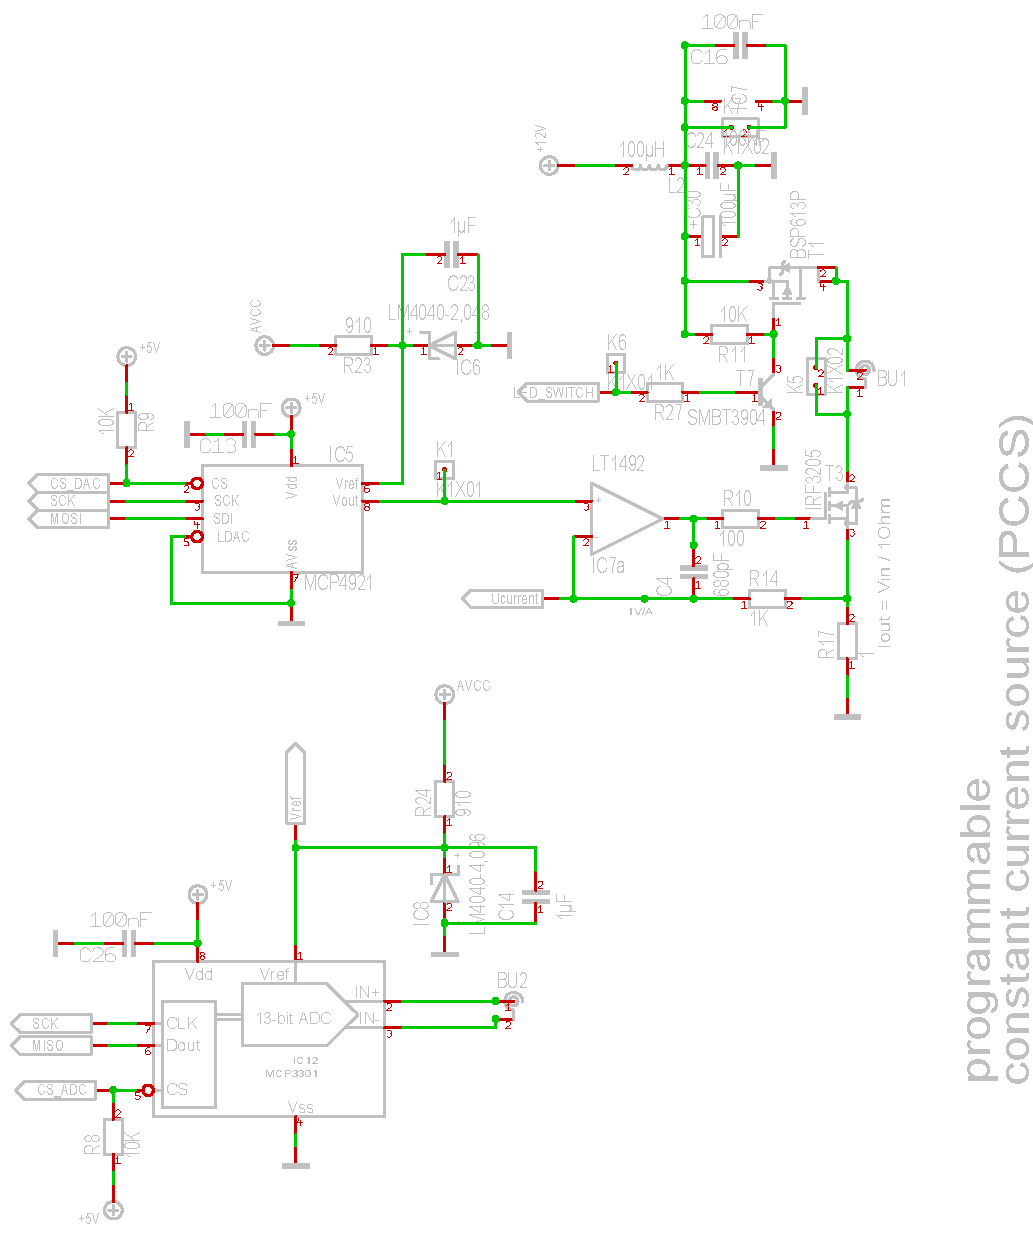
\includegraphics{schematic1.pdf}
	\caption{Schematic: Analog Part}
	\label{fig:schematic1}
\end{figure}

The PCCP circuit can be separated into three parts:
\begin{enumerate}
	\item \textbf{the analog part}, which controls the current through the LED, see Fig.~\ref{fig:schematic1}.\\The analog part consists of a DA converter (IC5), which is connected to an analog constant current sink (IC7a, T5). With T1, the LED can be switched on and off completely. The resolution of the DAC is approximately 1mA. The supply current is filtered with L2,C24,C30. Since the current sink is not set up as a switched-mode regulator, the excess power is converted to heat by T5. Therefor cooling of T5 should be added (with a heatsink and a fan, see Fig.~\ref{fig:schematic2}).\\In addition, the analog part contains an optional (!!!) AD converter (IC12), which can be used to measure any voltage in your setup. This circuit is NOT necessary for the operation of the basic power sink.
	\item \textbf{the digital part}, which contains the microcontroller, display, the USB connection and power-supply, see Fig.~\ref{fig:schematic2}.\\
	The digital part contains an ATmega microcontroller, which controls the analog part. The internal AD converter is used to read the current through the LED. In addition, the controller is connected to an LC display and four buttons, that allow to set the current through the LED. Also a serial-to-USB converter (IC2) is part of the circuit and allows for easy communication with a PC. The temperature sensor R13 and T2 are sued to build a temperature controlled fan controller to cool T5. The transistors T4/T5 constitute an optional digital output.
	\item a small circuit inside a \textbf{dongle}, which is specific to each LED. This dongle is a circuit, connected to a D-SUB 9-pole connector and basically contains an IIC EEPROM, which stores the LED parameters. This way, the circuit can read the LED parameter (max. current, name, ...) from this dingle and you can easily excahnge LEDs during operation: Just plug in the new LED and exchange the dongle. See Fig.~\ref{fig:schematic2} for teh schamtic.
\end{enumerate}

\begin{figure}[H]
	\centering
		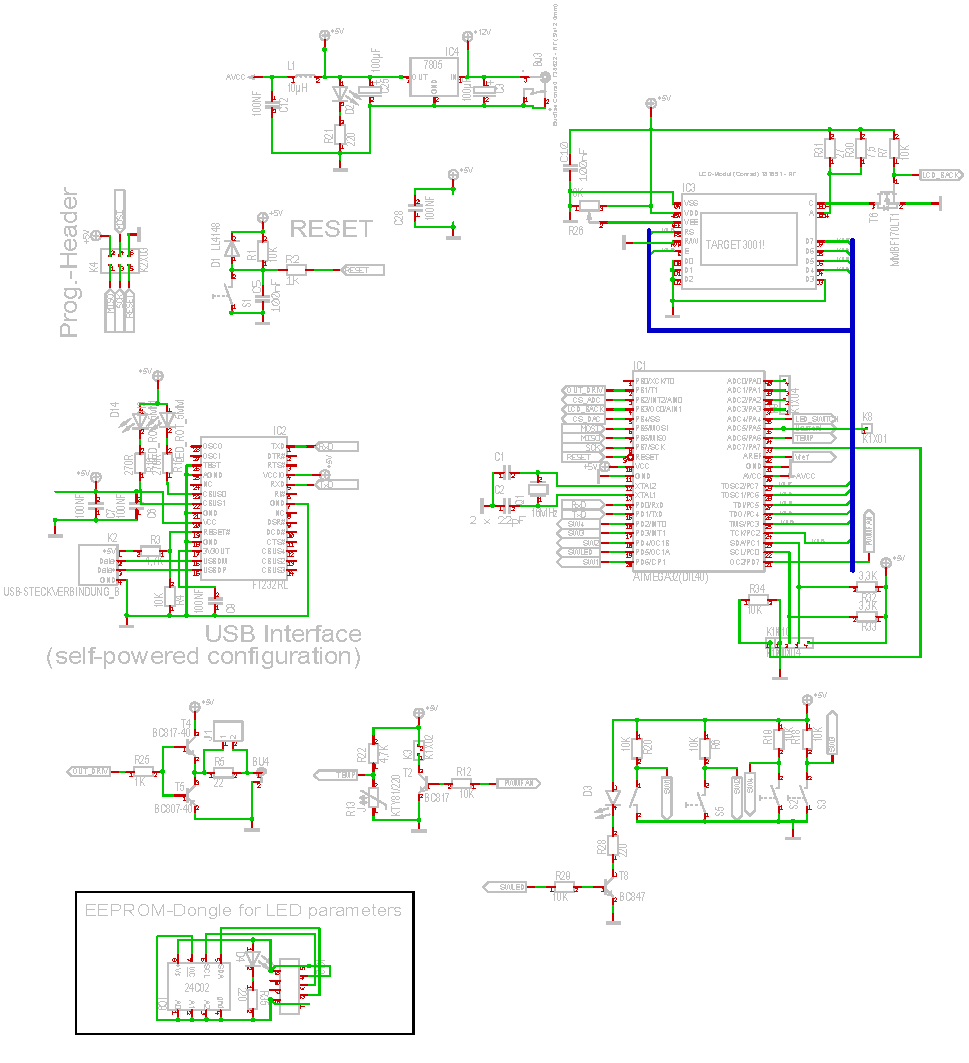
\includegraphics{schematic2.pdf}
	\caption{Schematic: Digital Part}
	\label{fig:schematic2}
\end{figure}


\subsection{PCB}
\label{sec:PCB}
\begin{figure}[H]
	\centering
		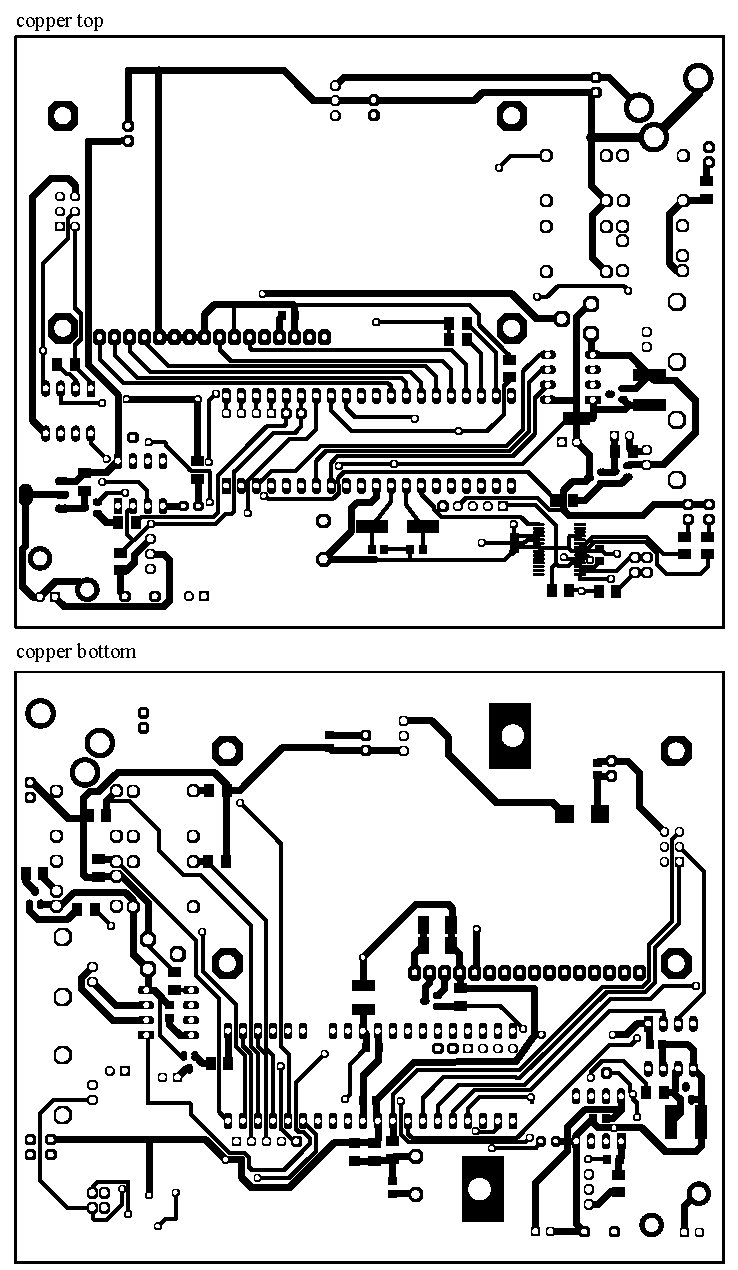
\includegraphics{boards.pdf}
	\caption{Board, top and bottom}
	\label{fig:boards}
\end{figure}
\begin{figure}[H]
	\centering
		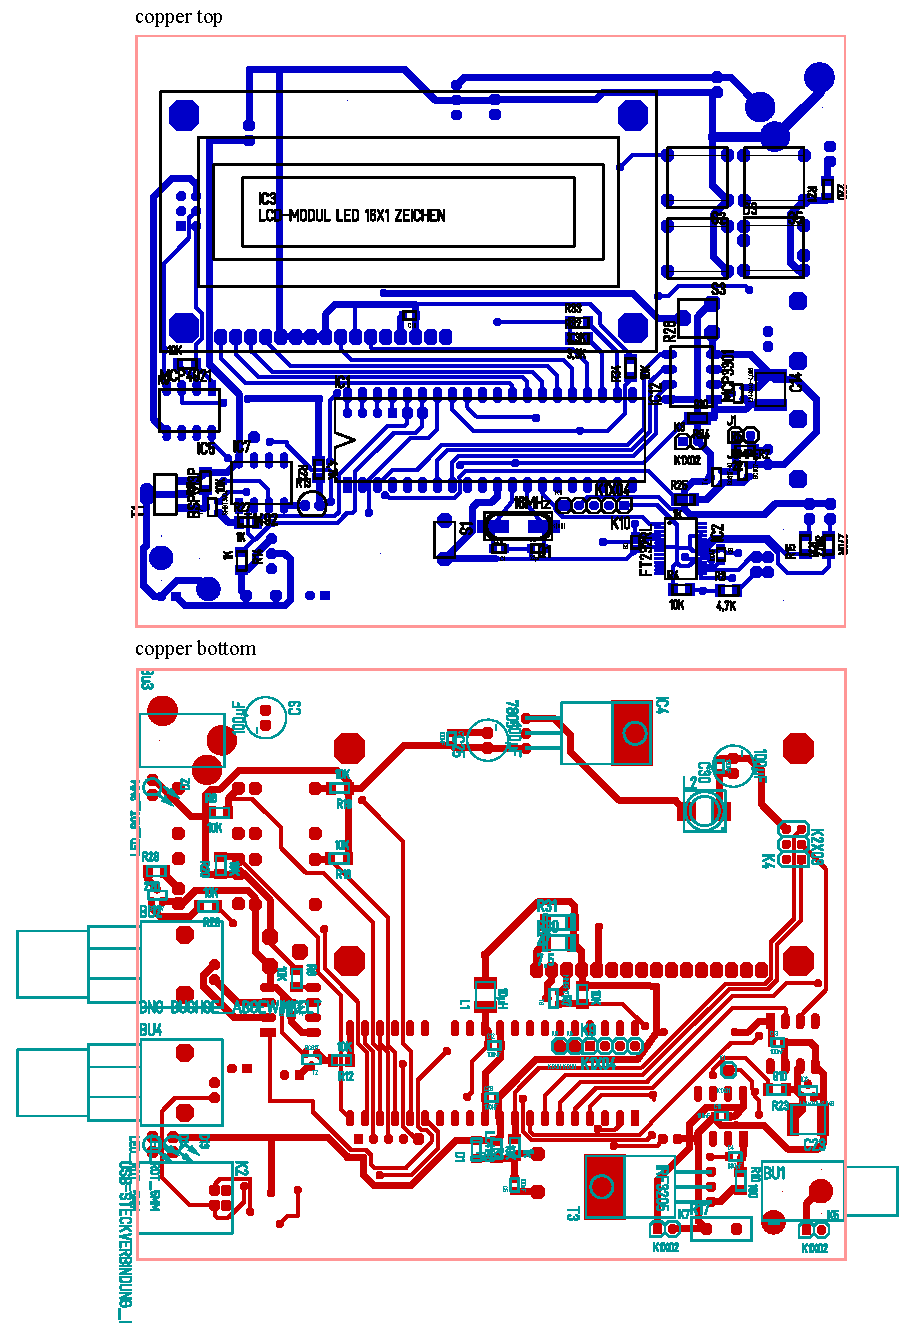
\includegraphics{boards_parts.pdf}
	\caption{Board, top and bottom, including parts}
	\label{fig:boards_parts}
\end{figure}


\subsection{Implementation Details and Hints}
\label{sec:ImplementationDetailsAndHints}
\begin{itemize}
  \item The FTDI USB to serial converter has areprogrammed device name 
		\begin{center}
			\textit{LASERBOX}
		\end{center}
		Still you can use the standard FTDI virtual COM port driver for this device: 
		\begin{center}
			\url{http://www.ftdichip.com/FTDrivers.htm}
		\end{center}

	\item The FTDI USB to serial converter has to be programmed to be self-powered. Otherwise the serial connection does not work on Linux (on Windows system the problem does not seem to exist).
	\item You can bind a box to a spoecific serial port. On \textbf{Windows} this can be done in the driver settings. On \textbf{Linux} this may be achieved using the \texttt{udev} hardware enumeration system:
	
\begin{enumerate}
	\item create a udev rules file with a name like e.g.: \texttt{/etc/udev/rules.d/99-laserboxes.rules} 
	\item add a line like this:

{\footnotesize\begin{verbatim}
  #LASERBox
  KERNEL=="ttyUSB*", SUBSYSTEMS=="usb", ATTRS{product}=="B040SERVO", SYMLINK+="ttyUSB_B040SERVO" 
\end{verbatim}}

    which will map the ttyUSB device with the product name B040SERVO to the device file \texttt{/dev/ttyUSB\_B040SERVO} in addition to its default file \texttt{/dev/ttyUSB}\textit{x}. Instead of the product name you can also use any other USB device property, as reported by

{\footnotesize\begin{verbatim}
  lsusb -v -s <bus>:<devnum>
\end{verbatim}}

    Possible filters are e.g.:

{\footnotesize\begin{verbatim}
   ATTRS{serial}=="A800dOBl", 
   ATTRS{idVendor}=="1a72", 
   ATTRS{idProduct}=="1007", 
   ATTR{vendor}=="0x149a", 
   ATTR{device}=="0x0005"
\end{verbatim}}

    \item After saving the rules file you will have to tell udev that there are new/changed rules by executing

{\footnotesize\begin{verbatim}
  /etc/init.d/udev restart
\end{verbatim}}

    The rules will be executed when the new device is connected to the computer. So if it's already connected: pull and reconnect the plug.

\end{enumerate}
\end{itemize}




\subsection{Programming the Laserbox Controller}
\label{sec:ProgrammingTheLaserboxController}
The main microcontroller of the control box is an Atmel ATmega32. It's flash memory may be programmed either by a standard AVR programmer, like usbasp (see \url{http://www.fischl.de/usbasp/} and Fig.~\ref{fig:usbasp}) or by a bootloader already installed on the controller. In the first case you should set the ``TargetSupply'' jumper of the usbasp and disconnect the power supply of the control box. This will supply 5V to the electronics of the control box which is OK for short periods (few minutes). Then you can use a programmer software like avrdude to program the controller. The programmer and the controller are connected by a standard $2\times3$ ribbon cable connectors (see Fig.~\ref{fig:pcb}).

If the controller is already equipped with the bootloader \texttt{avrprog\_boot v0.85} (by Martin Thomas, \url{http://www.siwawi.arubi.uni-kl.de/avr_projects#avrprog_boot}), you simply have to reset the controller (switch power off/on or use reset switch) while holding the ON/OFF button pressed down. Afterwards a new program can be loaded using a AVR109/AVR910 programmer software (e.g. avrdude, AVR Prog or AVR Studio) via the serial host port of the control box. Note that the bootloader is started only if the ON/OFF button is held down during a reset, otherwise the standard software starts and the control may be used to control a laser.

Here are some more hints on programming the controller:
\begin{itemize}
	\item The fuse bits for the ATmega324p controller without bootloader are: 
		\begin{center}
			\texttt{LFUSE = 0xFD;  HFUSE = 0xDF; EFUSE = 0xFF}.
		\end{center}
	\item The fuse bits for the ATmega324p controller with bootloader (2047 bytes) are: 
		\begin{center}
			\texttt{LFUSE = 0xFD;  HFUSE = 0xD8; EFUSE = 0xFF}.
		\end{center}
\end{itemize}


\begin{figure}[h]
	\centering
		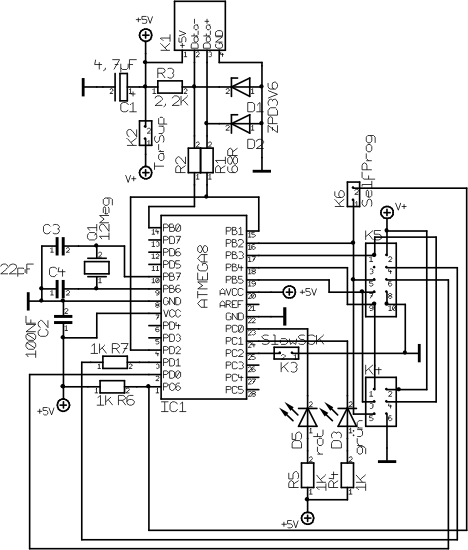
\includegraphics[width=100mm]{usbasp.png}
	\caption{USBasp -- AVR programmer for USB}
	\label{fig:usbasp}
\end{figure}




\newpage
\section{Literature \& Datasheets}
\label{sec:literature_datasheets}
\begin{itemize}
  \item FT232RL: \url{http://www.ftdichip.com/Documents/DataSheets/DS_FT232R.pdf}
\end{itemize}
\end{document}

